% arara: pdflatex: {shell: yes, synctex: yes, options: "-file-line-error-style"}
% arara: bibtex if found('log', 'undefined references')
% arara: pdflatex: {shell: yes, synctex: yes, options: "-file-line-error-style"}
% arara: pdflatex: {shell: yes, synctex: yes, options: "-file-line-error-style"}



% Before start, check the file README.txt
\documentclass[10pt,a4paper,twocolumn,english]{article}
\usepackage{sbsr}

%%%% This file presents the global settings for the document in LaTeX %%%%
%%%% (MORE INFORMATION IN README.txt) %%%%
%%%  The paper information must be declared below as well as its authors and affiliations %%%%

\title{Exploratory analysis of Recurrent deforestation warnings in 
São Félix do Xingu - Brazilian Amazon}

\author{Alber Sánchez Ipia$^1$, Guilherme Mataveli$^1$, Aline Pontes-Lopes$^1$ 
Sulimar Munira Caparoci Nogueira$^2$, and Luiz Aragão$^1$}

\address{$^1$Earth Observation and Geoinformatics Division - DIOTG, National 
Institute for Space Research - INPE, Av. dos Astronautas, 1758 - São José dos 
Campos - SP - Brazil alber.ipia@inpe.br, guilherme.mataveli@inpe.br, 
aline.lopes@inpe.br, luiz.aragao@inpe.br;
$^2$IDGeo - Inteligência Agrícola, suli.nogueira@gmail.com}

%%%% Beginning of the document %%%%

\begin{document}


% create the title %%%% (DO NOT CHANGE) %%%%
\twocolumn[
\begin{@twocolumnfalse}
\maketitle
\end{@twocolumnfalse}
]


%%%% Add each section file %%%%
%%%% (ALTER ONLY IF SECTIONS ARE INTRODUCED/REMOVED) %%%%

\section*{\textit {Abstract}} %%%% (DO NOT CHANGE) %%%%

\hspace{-1.5mm}\textit{ %%%% (DO NOT CHANGE) %%%%
%%%% Add the abstract below %%%%
%The abstract should appear at the top of the left-hand column of the text. The abstract should contain about 100 to 150 words. All manuscripts must be written in Portuguese, English or Spanish. Manuscripts must have a maximum of 4 pages including references.
Identifying forest degradation is as import as identifying deforestation, but 
even more challenging.
Due to the role of tropical forests in the Earth System, it is imperative to 
discover new ways to improve and characterize our knowledge about 
forest degradation.
This includes finding alternative uses for already existing data such as the 
warnings issued by the DETER system.
In this paper, we explore the DETER warnings in \textit{São Félix 
do Xingu} from 2016 to 2021 and compute their frequency over the same areas.
We found forest areas with up to 4 warnings 4 years apart and their mean time
between the first and second warnings is two years and one year between the 
second and the third.
Our results are important because they point to DETER as a source of data for 
analyzing the development of deforestation by recurrent degradation.
}
\\

%%%% Add the Key words below %%%%
\textit{\textbf{Key words --} %%%% (DO NOT CHANGE) %%%%
Degradation, Deforestation, DETER. %%%% (ADD KEY WORDS) %%%%
}



\section{Introduction}

% Background, known information.
The Amazon forest plays an important role in the current climate crisis.
Besides hosting a large number of species and regulating the water and carbon 
cycles, the forest works as a large carbon storage and it is frequently cited  
as one of the tipping points, which ---if mishandled--- could potentially cause 
an abrupt and irreversible change in the climate 
system~\cite{rockstrom2009,armstrong2022}.

% Knowledge gap, unknown information.
Advances in the areas of Ecology, Remote Sensing, and Computer Science have
fostered regional, continental and even global deforestation
monitoring systems (e.g. PRODES, Global Forest Watch).
However, detecting forest degradation is more challenging than detecting
deforestation~\cite{lambin1999,mitchell2017}.

% Hypothesis, question, purpose statement.
Due to the importance of what is at stake, we seek new ways to improve 
degradation characterization which could alleviate the difficulties 
associated to detection of forest degradation.
For this reason, in this manuscript, we explore the possibilities of using 
DETER warnings for understanding forest degradation.
DETER constantly issues deforestation warnings on the Brazilian Amazon forest, 
and these warnings capture forest degradation at different stages of
development.
This information has many potential applications, such as for example, 
providing quality training data for Machine Learning algorithms able to process 
massive amounts of satellite imagery.

% Approach, plan of attack, proposed solution.
To test the feasibility of our approach, we processed 5 years of DETER 
warnings in the municipality of \textit{São Félix do Xingu}, estimating the 
areas and number of days between warnings on the same area.


\section{Material e methods}

For our analysis, we selected the municipality of \textit{São Félix do Xingu} 
in the Brazilian state of \textit{Pará} as our area of interest in the period 
from August 2016 to July 2021. 
This municipality extent is 82 square kilometers and it is consistently 
reported as one of the most deforested in 
Brazil by the PRODES system~\cite{f.g.assis2019}.

We prepare a dataset of degradation and deforestation warnings produced by the 
Brazilian National Institute for Space Research (INPE) and its DETER system.
DETER is a Geographic Information System which produces a fast assessment of 
forest degradation and deforestation in the Brazilian Amazon since 
2004~\cite{shimabukuro2006}. 
DETER is the backbone of law enforcement efforts in the Brazilian Amazon and 
Cerrado Biomes.
Since 2015, DETER uses remote sensing imagery captured by the WFI camera
on board of the CBERS 4 \& 4A satellites, producing warnings 
with a minimum area of 3 ha organized into classes: Wildfire scar, mining, 
deforestation with either exposed soil or vegetation, degradation, and 
selective cut with either disordered or geometric 
pattern~\cite{diniz2015,f.g.assis2019}. 
To spot deforestation, DETER employs human experts which use image composition 
of red, near-infrared, and green along with a Linear Mixture 
Model~\cite{shimabukuro1991} (soil fraction) and the criteria of tone, color, 
shape, texture, and context. 
These experts draw DETER warnings on top a computer screen fix on a scale 
1:100,000 using as background the latest PRODES primary forest mask and 
previous DETER warnings~\cite{dealmeida2022}.


Our data set consists of the warnings issued in our area of interest during the
aforementioned period downloaded from the TerraBrasilis 
portal~\cite{f.g.assis2019}. 
After downloading the data, we convert them into a 
GeoPackage;~\footnote{GeoPackage Encoding Standard 
\url{https://www.ogc.org/standards/geopackage}} this helps us overcome the 
limitations~\footnote{Switch from Shapefile 
\url{http://switchfromshapefile.org/}} of the traditional Shapefile format 
available from INPE. 

Then, it was used the self-intersect operation (union operation) on the warning 
polygons and after that, we projected them to the coordinate reference system 
UTM 22s; later, we removed duplicated vertices and enforced the right-hand-rule 
of polygons; then we applied successive geometry fixing, and finally we 
filtered out polygons smaller than 3 ha. 
These operations were applied using the software QGIS version 
3.28.0~\cite{QGIS_software}.
We also converted the warning year to what we call PRODES year, which is time 
period from August to July. Each PRODES year takes the year number from the 
last month of its period (July).

It is important to note that DETER warnings overlap over time but not
completely. That means, some segments of a warning partially overlap with 
some other segments of other warnings at other dates.
We call the result of the self-intersect operation \textit{subareas} and they 
correspond to segments of DETER warnings which, if overlap other subareas, 
they do have the same spatial properties (position, area, shape, and centroid).

Finally, we used the GNU's R language and environment for statistical 
computing and graphics to estimate statistics and carry on further 
analysis~\cite{r_manual}. 
The source code of our analysis is available 
online.~\footnote{File sbsr\_2013.R available at
\url{https://github.com/albhasan/treesburnareas}}



	
\section{Results}

\textit{São Félix do Xingu} has a growing trend of DETER warnings from August 
2016 to July 2021, where 2018 presents a particularly worrying peak. There are increases
in the warning areas of DETER along all sizes (see 
Figure~\ref{fig:deter_warnings_area_size}).

\begin{figure}[h] 
    \begin{center}
    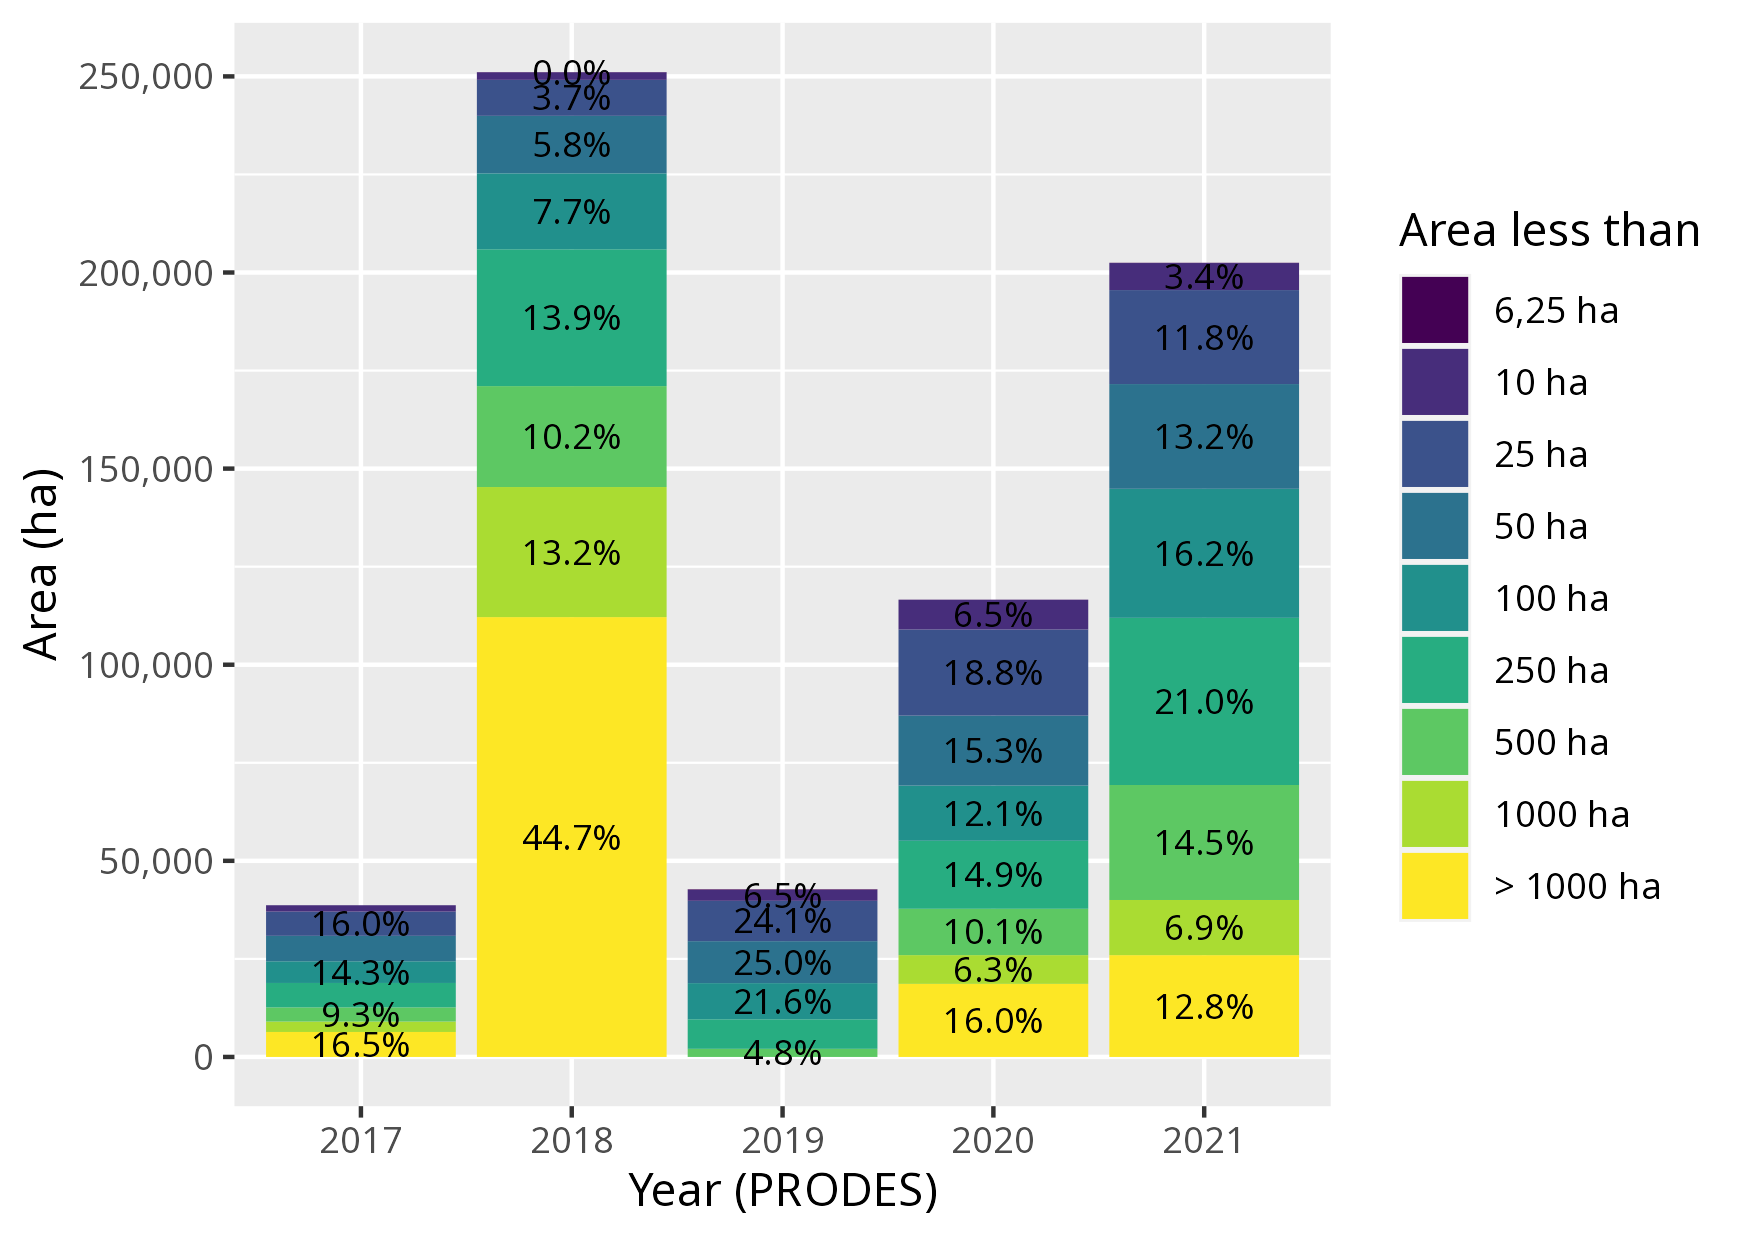
\includegraphics[width=\linewidth]{deter_warnings_area_size.png}
    \caption{Area of DETER warnings by year and size. The area covered by 
        warnings peaked in 2018. Note the increasing trend since 2019
        and how their distribution is homogeneous along the size brackets in 
        2021.}
    \label{fig:deter_warnings_area_size}
    \end{center}
\end{figure}

Meanwhile, the number of DETER warnings displays the same growing trend except
for the 2018 peak that isn't very prominent, indicating an increment not only 
in the number of DETER warnings, but also in their size (see 
Figure~\ref{fig:deter_warnings_size}).

\begin{figure}[h] 
    \begin{center}
    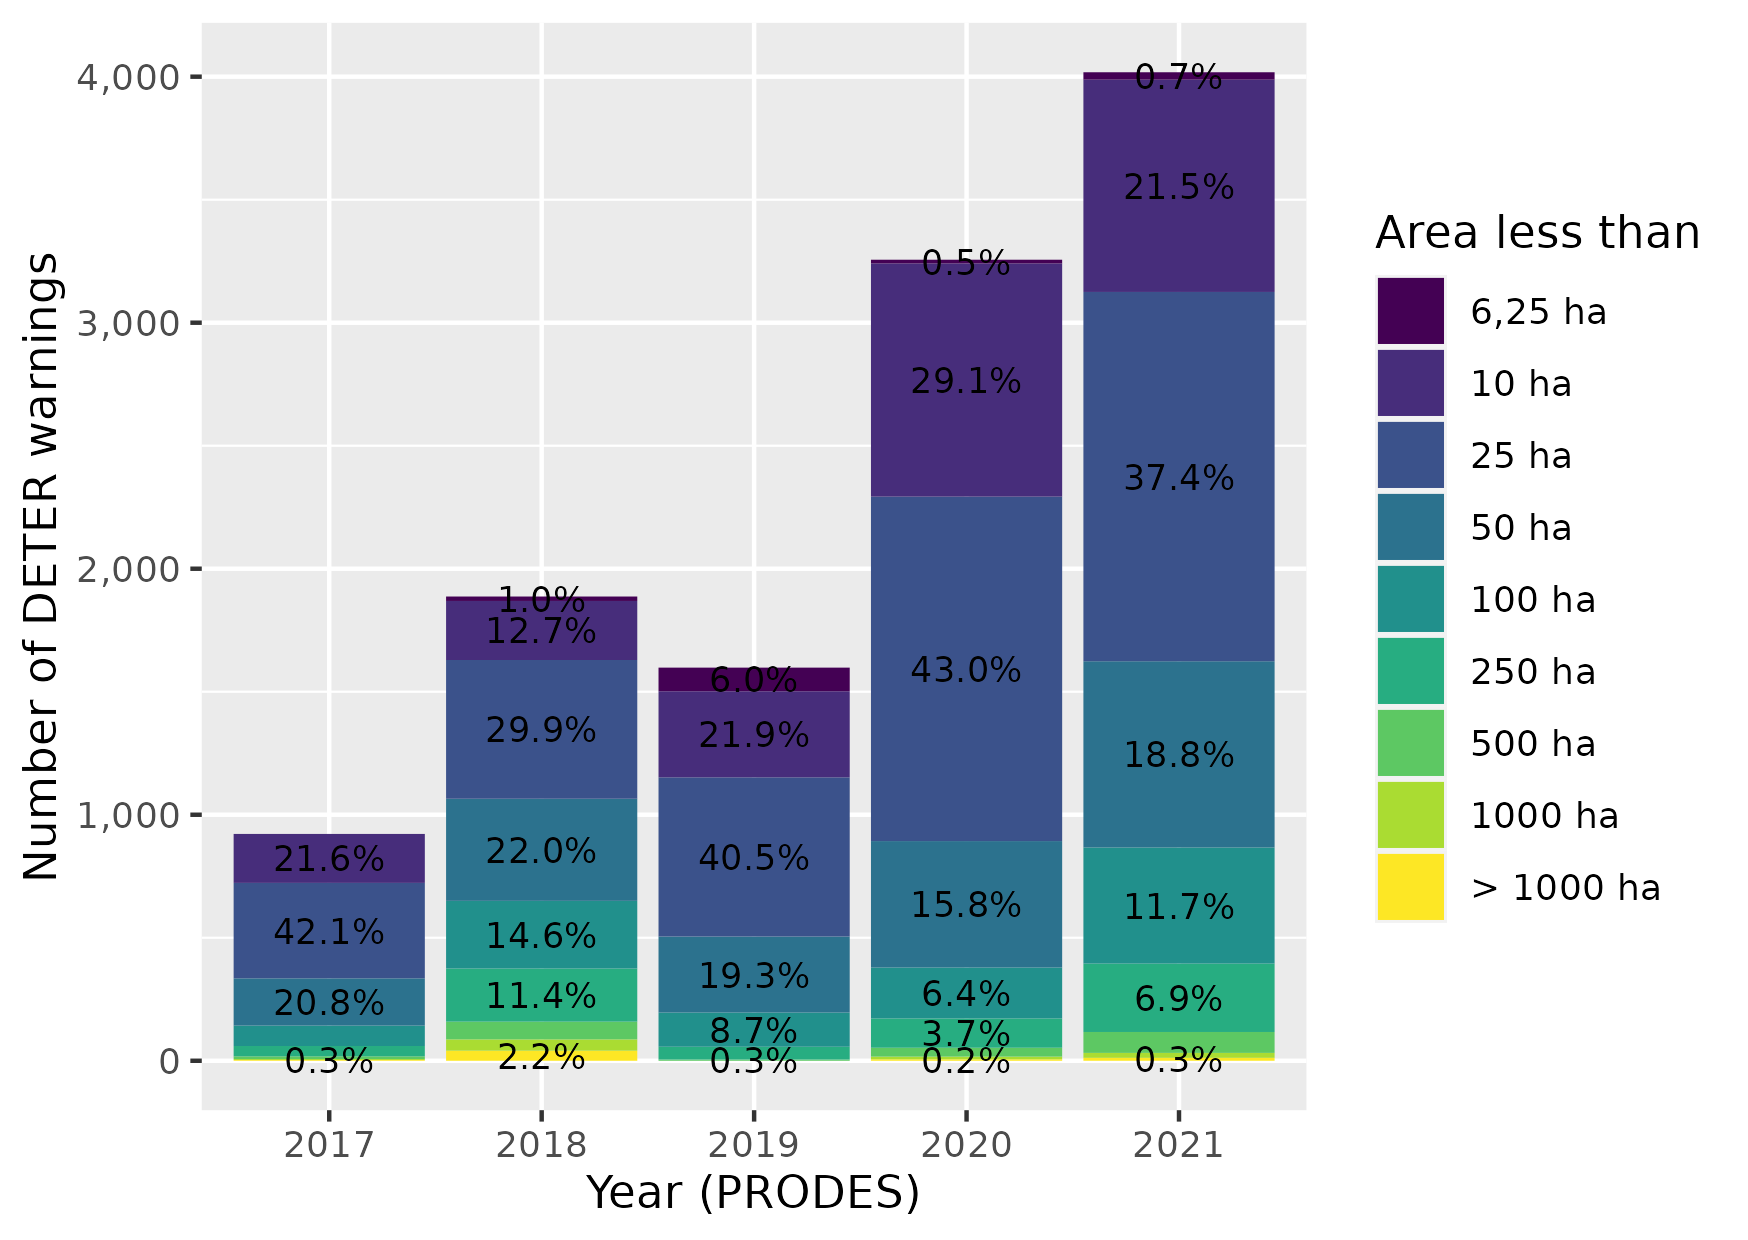
\includegraphics[width=\linewidth]{deter_warnings_size.png}
    \caption{Number of DETER warnings by year and size.Note the increasing 
        trend since 2017. The increase in warnings in 2018 corresponds to a
        large increase in area, implying an increment in the size of each 
        warning.}
    \label{fig:deter_warnings_size}
    \end{center}
\end{figure}

The month where most DETER warnings are issued in the area of interest during
the study period is September (the end of the 2-month dry season in half of the
Amazon~\cite{carvalho2021}), followed by October and August.
The yearly increasing trend is also found inside September and October (even 
the 2018 peak), the months with the most warnings, (see 
Figure~\ref{fig:deter_warnings_size_month}). 

\begin{figure}[h] 
    \begin{center}
    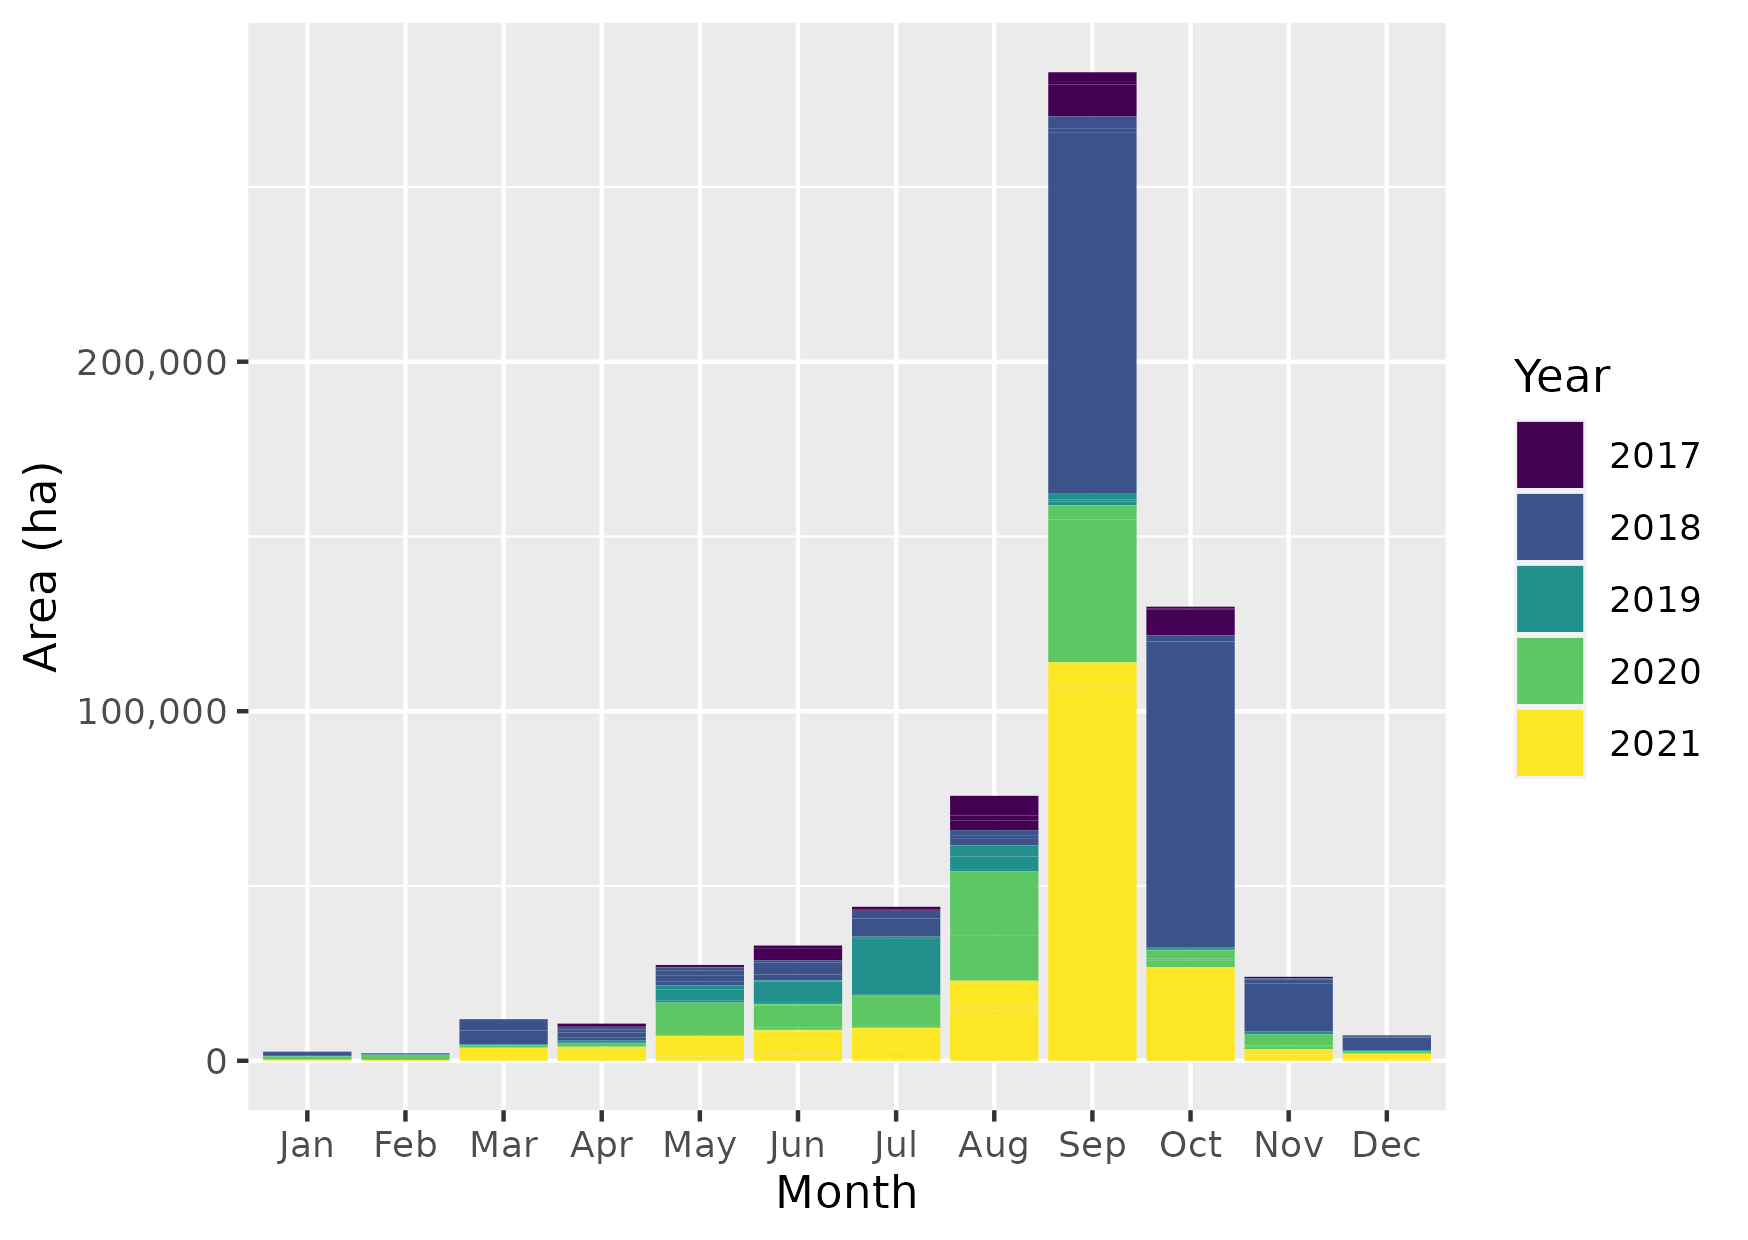
\includegraphics[width=\linewidth]{deter_warnings_size_month.png}
    \caption{DETER warnings by month. Between August and October is when most
        of the warnings are issued. Note how September presents an increasing 
        trend along the years on which 2018 is comparable to 2021.}
    \label{fig:deter_warnings_size_month}
    \end{center}
\end{figure}

Our analysis also shows that most subareas in the area of study receive only 
one DETER warning (see Figure~\ref{fig:plot_area_by_warnings}) and those which 
receive a second one, they receive it two or three years after (see 
Figure~\ref{fig:plot_days_first_to_last} and 
Table~\ref{tab:warnings_subareas_by_number_area}). 
% NOTE: Why aren't they receiving their second warnings one year after?
The remaining subareas, which receive a third or even a fourth waning, receive 
their last warning between three and four years after the first one (see 
Figure~\ref{fig:plot_days_first_to_last}).

\begin{figure}[h] 
    \begin{center}
    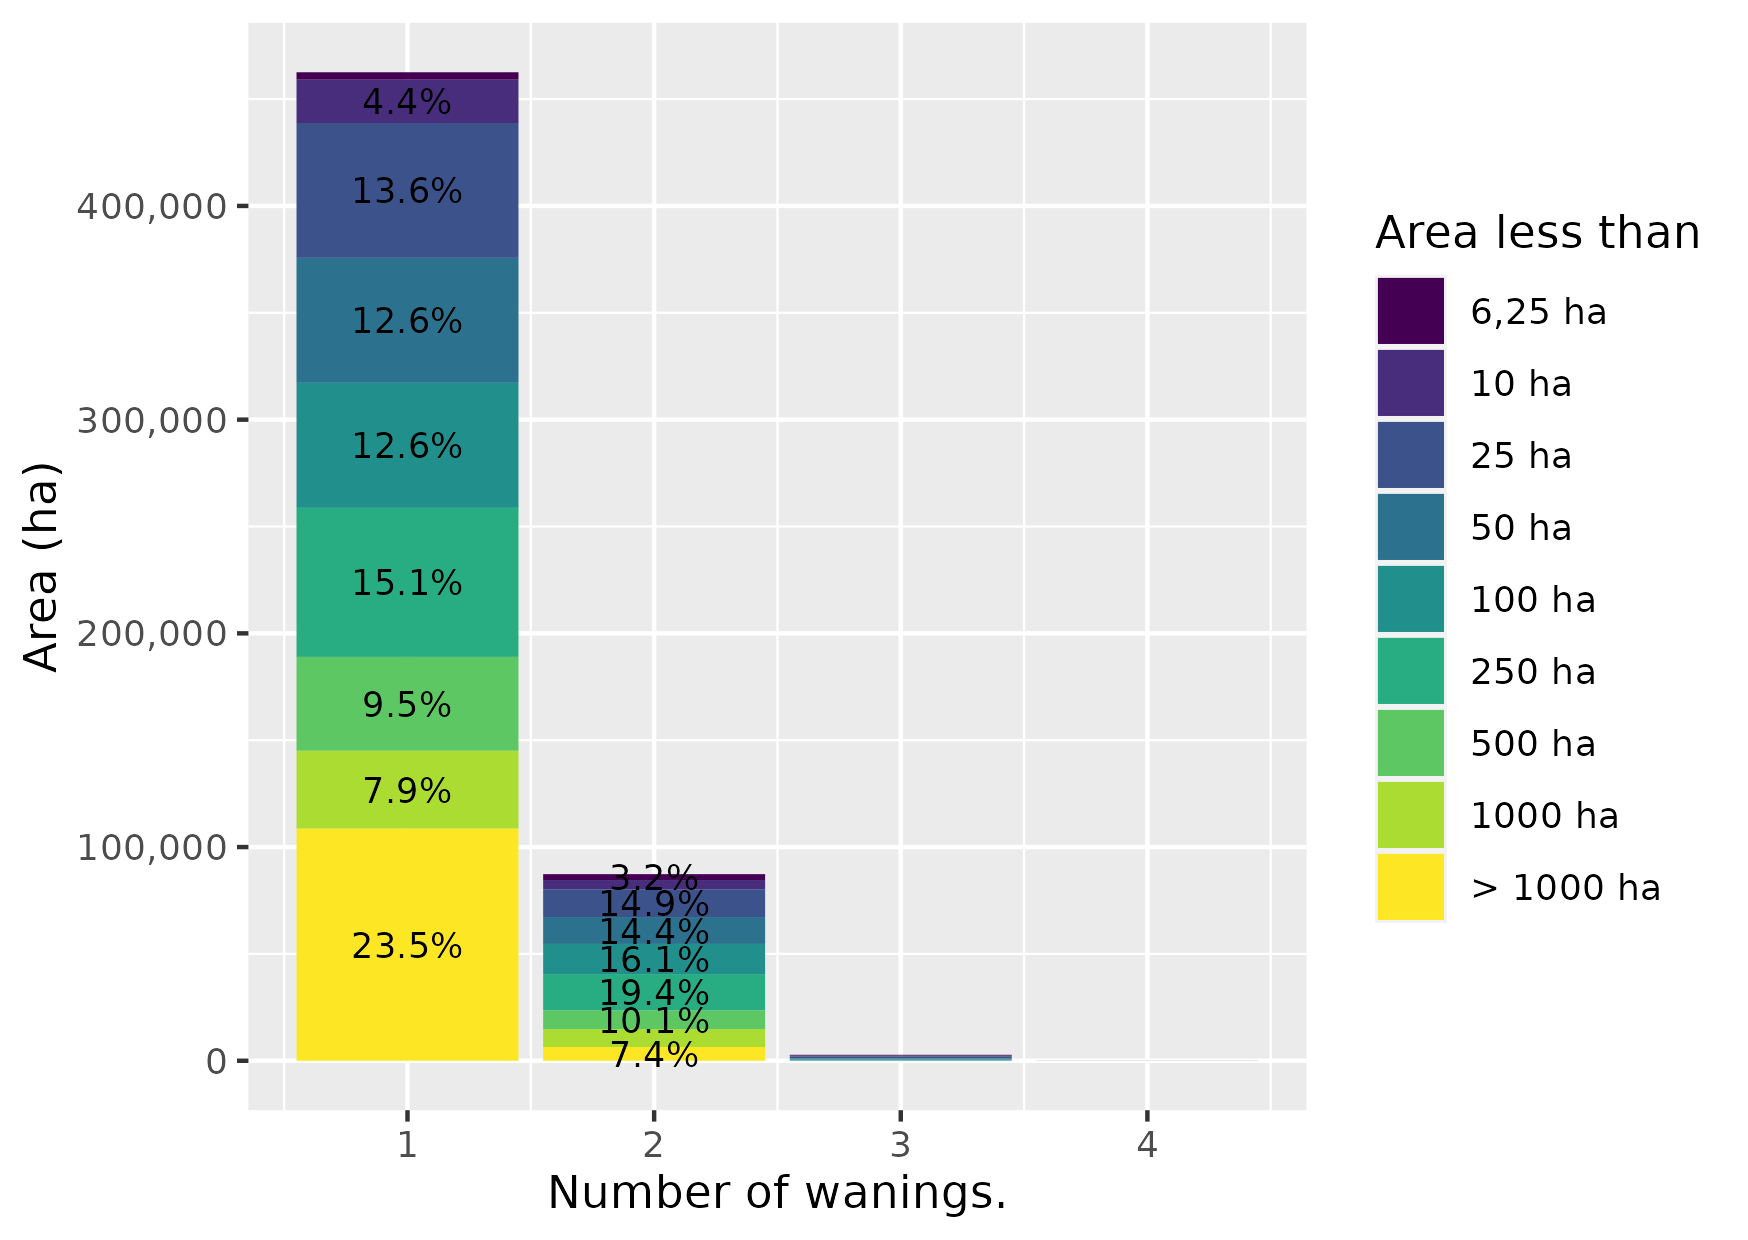
\includegraphics[width=\linewidth]{plot_area_by_warnings.png}
    \caption{DETER warning area by number of warnings. Most subareas are issued
        a DETER warning only once, and never more than four.}
    \label{fig:plot_area_by_warnings}
    \end{center}
\end{figure}

\begin{table}[h] % use [t] here to force table to top
    \centering
    \begin{tabular}{|c|c|r|r|}
        \hline
        \textbf{N. Warnings} & \textbf{Type} & 
        \textbf{N. Subareas} & \textbf{Total area}  \\
        \hline
1 & 6.25 ha    &  749  &   3468.9 \\ 
1 & 10 ha      & 2535  &  20277.6 \\
1 & 25 ha      & 4002  &  63098.2 \\
1 & 50 ha      & 1682  &  58496.4 \\
1 & 100 ha     &  847  &  58490.3 \\
1 & 250 ha     &  459  &  69741.0 \\
1 & 500 ha     &  133  &  43890.2 \\
1 & 1000 ha    &   54  &  36388.0 \\
1 & > 1000 ha &   42  & 108701.0  \\
        \hline
2 & 6.25 ha    &  617  &   2754.4 \\
2 & 10 ha      &  542  &   4300.3 \\
2 & 25 ha      &  829  &  13016.6 \\
2 & 50 ha      &  356  &  12588.7 \\
2 & 100 ha     &  200  &  14101.6 \\
2 & 250 ha     &  111  &  16949.5 \\
2 & 500 ha     &   25  &   8804.5 \\
2 & 1000 ha    &   12  &   8361.2 \\
2 & > 1000 ha &    3  &   6444.0  \\
        \hline
3 & 6.25 ha    &   70  &    331.8 \\
3 & 10 ha      &   48  &    383.2 \\
3 & 25 ha      &   62  &    943.4 \\
3 & 50 ha      &   15  &    528.5 \\
3 & 100 ha     &    5  &    342.0 \\
3 & 250 ha     &    2  &    261.5 \\
        \hline
4 & 6.25 ha    &    5  &     24.4 \\
4 & 10 ha      &    1  &      8.4 \\
4 & 25 ha      &    2  &     31.4 \\
        \hline
    \end{tabular}
    \caption{DETER warning subareas by number of wanings, type, number of 
    subareas, and total area. The number and total area decreases as the number
    of warnings increase.}
    \label{tab:warnings_subareas_by_number_area}
\end{table}


Besides, subareas smaller than 50 or 100 ha and two DETER warnings tend to 
receive their second waning two years after the first while larger subareas 
tend to receive them after three years (see the medians in 
Figure~\ref{fig:plot_days_first_to_last}). 
Something similar happens to subareas with 3 warnings, where subareas smaller 
than 25 ha receive their last warning approximately one year before than larger 
subareas.

\begin{figure}[h] 
    \begin{center}
    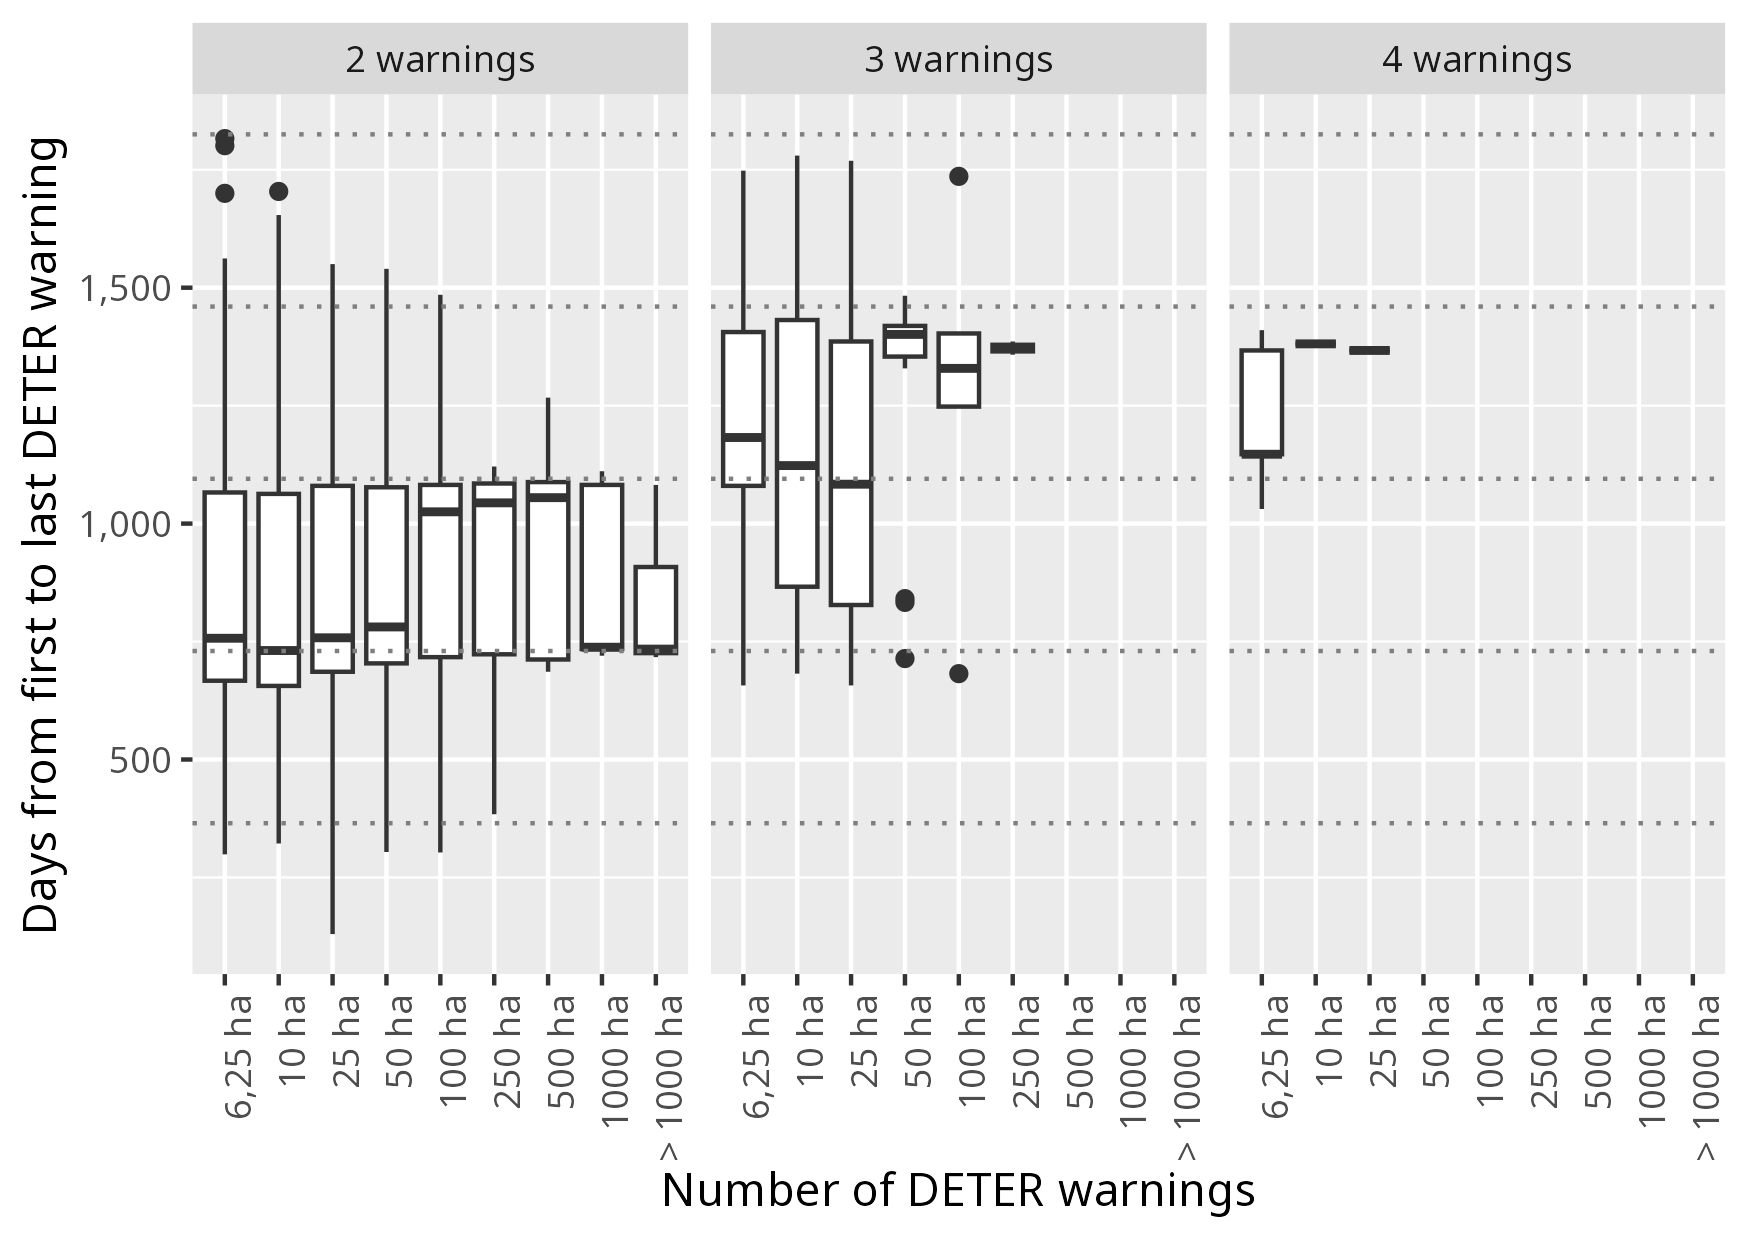
\includegraphics[width=\linewidth]{plot_days_first_to_last.png}
    \caption{Number of days between the first and last DETER warning of the 
        same subarea. Note how the difference between 2 and 3 warnings is 
        approximately 365 days (dotted lines). Each Box plot shows the median; 
        the first and third quartiles (hinges); 1.5 times the inter-quartile 
        range from the hinges; and the outliers.}
    \label{fig:plot_days_first_to_last}
    \end{center}
\end{figure}


	
\section{Discussion}

Our results show that the number of subareas with more than one DETER warning
is low compared to the total number of warnings and there are but a few of 
subareas with more than three warnings.
They also show that most of successive warnings of the same subarea are at most 
four years apart, two years from the first to the second, and one year from 
there. 
We found that DETER warnings provide between two and four warnings to 
characterize degradation processes in one of the most deforested municipalities 
in the Amazon. 

The number of available subareas seems small for training Machine Learning 
algorithms, specially those based on Deep Learning that are well-known
for requiring large amounts of training data.
However, we expect these numbers increase by extending our analysis to the 
whole area covered by the Brazilian Amazon since 2016.
In addition, we think our results foster new analysis in areas different from 
Computer Science.
Despite this fact, our results are important as they explore a potential new
application of the already useful and openly available DETER data.

Our results rely on the assumption that \textit{São Félix do Xingu} is 
representative of degradation in the Amazon.
They also rely on the accuracy of DETER warning polygons and the assumption
that subareas larger than 3 ha correspond to actual degradation warnings 
instead of drawing inaccuracies on a computer screen.


	
%\section{Conclusions}

%Major headings, for example, "1. Introduction", should appear in all capital letters, bold face, centered in the column, with one blank line before, and one blank line after. Use a period (".") after the heading number, not a colon.

%If the last page of your paper is only partially filled, arrange the columns so that they are evenly balanced if possible, rather than having one long column.

%List and number all bibliographical references at the end of the paper.  The references can be numbered in order of appearance in the document.  When referring to them in the text, type the corresponding reference number in square brackets as shown at the end of this sentence \cite{Smith_year}.

%To insert citations in \LaTeX, use {\small \verb|\cite{<author>}|}, which produces ``\cite{Jones_year} ''. The bibliography is located in file {\small \verb|07_SBSR.bib|}. The references are automatically generated.

TODO.


\section{Acknowledgements}

The authors would like to acknowledge the Conselho Nacional de Desenvolvimento 
Científico e Tecnológico (CNPq Projeto: 444418/2018-0, Processo: 350820/2022-8). 
Guilherme Mataveli was financed by the São Paulo Research Foundation (FAPESP, 
grant 2019/25701-8).
Aline Pontes-Lopes was also financed by FAPESP (grant 22/04893-9).

 
%%%% Create the references below (DO NOT CHANGE) 
%%%% (MORE INFORMATION IN README.txt) %%%%

%%%%%%%%%%%%%%%%%%%%%%%%%%%%%%% ATTENTION %%%%%%%%%%%%%%%%%%%%%%%%%%%%%%%%
%%%% The file extra considerations (extra_considerations.tex) is not part of the template and must be removed from the final work. To do so, comment the line below %%%%
%\section{PAGE NUMBERING}
    
Please do \textbf{not} paginate your paper. Page numbers and conference identification will be inserted when the paper is included in the proceedings.
\pagebreak
	
\section{Illustrations, graphs, photographs and tables}
	
Illustrations must appear within the designated margins. If needed, figures may span the two columns. If possible, position illustrations at the top of columns, rather than in the middle or at the bottom. Caption and number every illustration (Figure \ref{example_figure}). The same rules apply to tables (Table \ref{example_table}). 
	
\begin{figure}[h] % use [t] here to force figure to top
    \begin{center}
    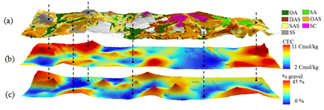
\includegraphics[width=\linewidth]{figures/example_figure.png}
    \caption{Figure caption (and also Table caption) must have a font 9 and be in bold.}
    \label{example_figure}
    \end{center}
\end{figure}

\begin{table}[h] % use [t] here to force table to top
    \centering
    \begin{tabular}{|c|c|c|c|}
        \hline
        \textbf{Item 1} & \textbf{Item 2} & \textbf{Item 3} & \textbf{Item 4}  \\
        \hline
        Value 11 & Value 12 & Value 13 & Value 14  \\
        \hline
        Value 21 & Value 22 & Value 23 & Value 24  \\
        \hline
    \end{tabular}
    \caption{Rules for table caption are the same as figures.}
    \label{example_table}
\end{table}
 

\renewcommand{\refname}{REFERENCES}
{\small
\bibliographystyle{unsrt} 
\bibliography{07_SBSR.bib}}
	
\end{document} % end of document %%%%(DO NOT CHANGE)%%%%
